\chapter{
    \textbf{Introduction}
}
\section{Data Hiding}
\justifying{
    \large{
        \paragraph{} \textit{Information security} is the field of Computer Science which deals with the protection of sensitive information from access, use and modification by unauthorised users. The practices of information security are commonly divided into two - \textit{Cryptography} and \textit{Data Hiding}. While cryptography deals with the transmission of information in encrypted forms, data hiding hides the existence of secret communication.
        \paragraph{} In data hiding, secret messages are usually hidden inside a carrier cover file, which can be a text file, image file, audio file or video file. Image files are popularly used for data hiding but recently, video files have also gained popularity due to its high data hiding capacity.
        \paragraph{} Data hiding methods are commonly of three types: 
        \begin{itemize}
            \item Watermarking
            \item Steganography
            \item Reversible Data Hiding
        \end{itemize}
    }
}
\begin{figure}
    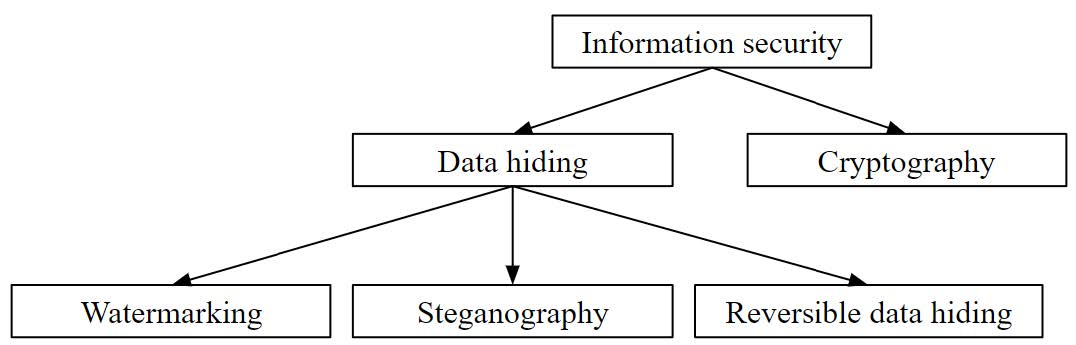
\includegraphics{images/1.jpg}
    \caption{Different Data Hiding Techniques} 
\end{figure}
\section{Steganography}
\justifying{
    \large{
        \paragraph{} Steganography is the practice of concealing information within another non-secret file or message in such a manner that the presence of information is not evident to human inspection. Steganography can also be combined with an extra step of encryption for an additional layer of security. There are four common types of steganography as given below.
        \\[2\baselineskip]
        \begin{figure}
            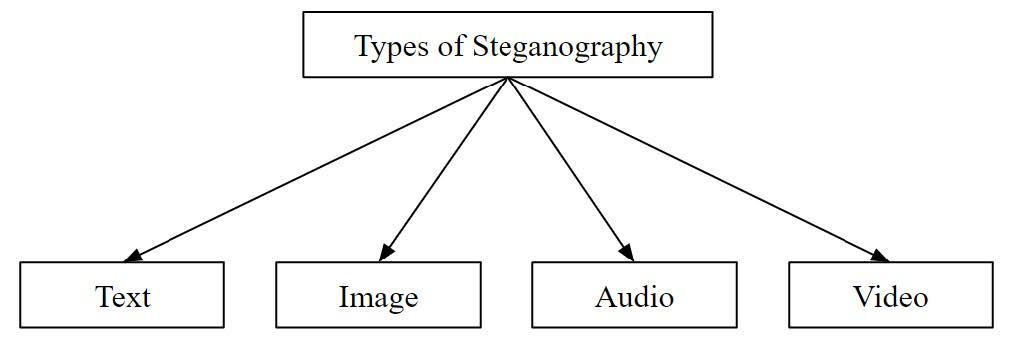
\includegraphics{images/2.jpg}
            \caption{Types of steganography}    
        \end{figure}
        \paragraph{} Although image steganography is considered to be very popular and has been widely used for the transmission of secret messages, recent trends show the use of video steganography for covert communications due to its high data hiding capacity.
    }
}
\section{Video Steganography}
\justifying{
    \large{
        \paragraph{} Video steganography is the practice of hiding secret data inside an ordinary non-secret video file. Any type of digital content can be hidden inside a video file and hence, it is preferred over other steganographic methods. Secret data inside a cover video file, called a stego video, is sent via common transmission media and is extracted at the destination using various techniques. The cover video file used could either be a raw video file or a compressed video file depending on the capacity of the secret data and the speed of transmission. \\
        \centering
            \begin{figure}[h]
                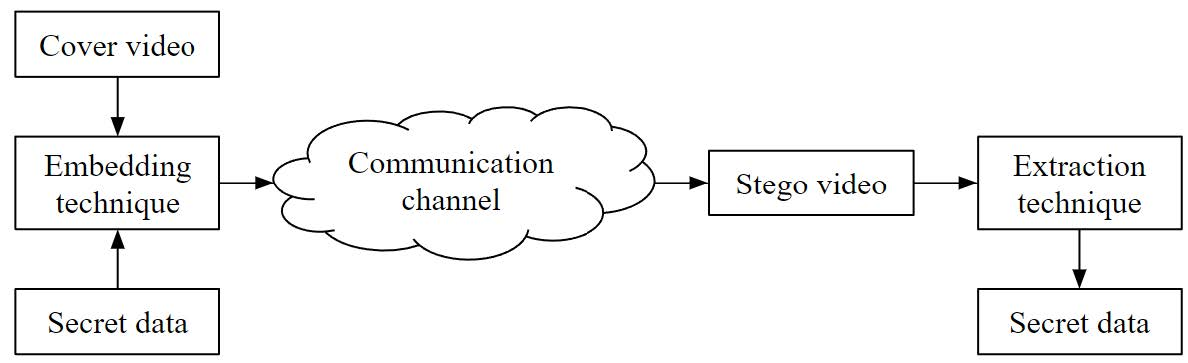
\includegraphics{images/3.jpg}
                \caption{Process of video steganography}    
            \end{figure}
        \paragraph{} The desirable features of a video steganography method are:
        \begin{itemize}
            \item High embedding capacity
            \item Low complexity
            \item Good visual quality
            \item Less vulnerability
            \item Effective frame selection
        \end{itemize}
    }
}
\section{Existing Techniques}
\justifying{
    \large{
        \paragraph{} Video steganography methods that focus on the spatial domain of the video file are commonly of two types:
        \begin{enumerate}
            \item LSB methods: In LSB-based methods, the secret message is embedded by changing the least significant bit value/values of the related pixel.
            \item ASCII coding methods: In ASCII coding methods, the secret message is converted to ASCII code and is directly hidden to the last digit of the relevant pixel.
        \end{enumerate}
        \paragraph{}A special type of LSB method known as LSB 3-3-2 method embeds 8-bit secret data into three least significant bits of the red channel, three of the green channel and two of the blue channel. LSB332 is found to be more effective than other LSB-based methods in terms of visual quality of the stego video.
    }
}